\section{Continuous and Discrete Traffic Model for Freeway Control}
\label{sec:continous-and-discrete-traffic-model-for-ramp-metering}

In this section, we derive and motivate the continuous freeway network traffic model and discuss its improvements over existing models. We also present the discretized version of the continuous model, which is used extensively in applications in the remainder of the thesis. 

\subsection{LWR Equation}

The Lighthill-Whitham-Richard (LWR) equation~\cite{lighthill1955kinematic,richards1956shock} is a scalar conservation law used to represent the evolution of vehicle density on a section of linear roadway. The distinguishing assumptions in the LWR model deal with the flux function, $f\left(\rho\right)$, referred to as the \emph{fundamental diagram of traffic}. Namely, we assume the following rules on $f$:

\begin{enumerate}
	\item $f\left(\rho \right) = \rho v\left(\rho \right)$, where $v$ is the velocity of the vehicle density.
	\item $v\left(\rho \right)$ is a decreasing function of $\rho$.
	\item $f$ is defined over the values $\left[0,\rho^{\max}\right]$, where $\rho^{\max}$ is considered the \emph{jam} density.
	\item $f\left(0\right) = f\left(\rho^{\max}\right) = 0$.
\end{enumerate}

The four rules above fit well with our intuition of road traffic. Rules 1 and 2 state that the flux varies as the velocity varies, and that as the roadway gets more congested, the speed of the vehicles will only decrease. Rule 3 fits with the physical interpretation of vehicle as being non-negative, and that there must be an upper limit of vehicle density (due to minimum car lengths). Rule 4 states that no vehicles will have no flow, and that flow completely breaks down at the maximum density.

\begin{figure}[htbp]
	\centering
	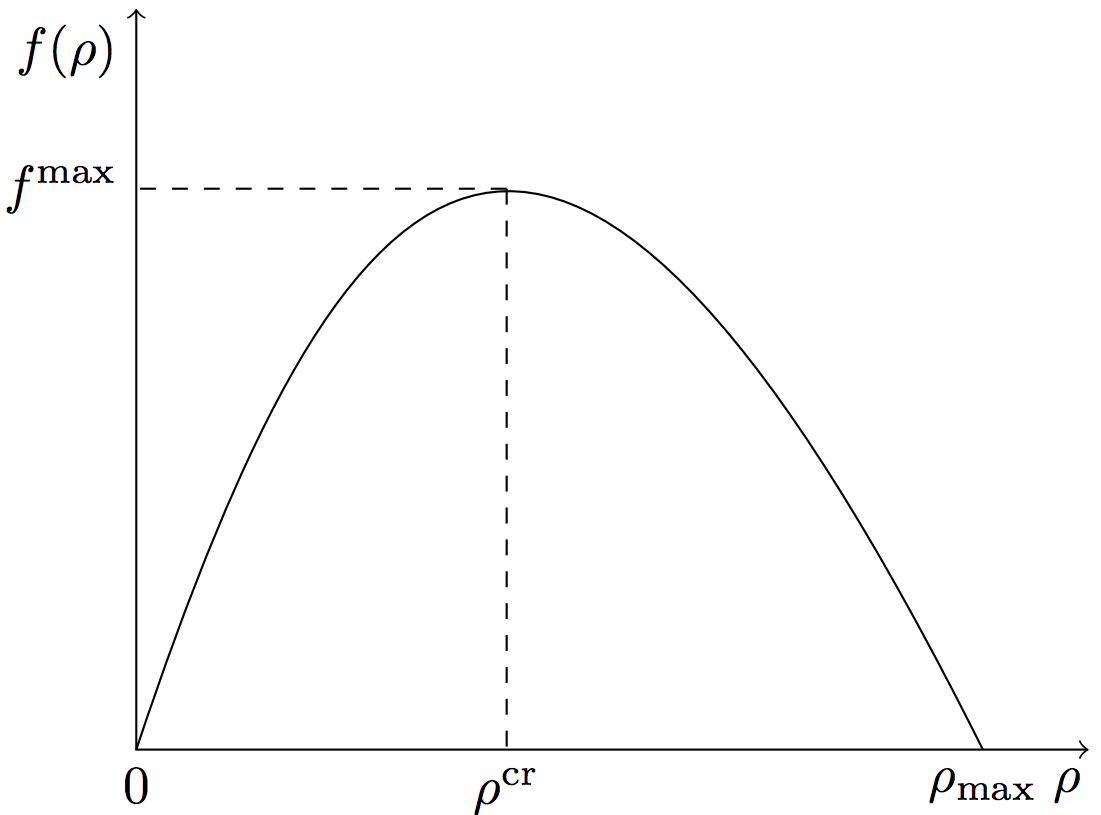
\includegraphics[width=0.6\textwidth]{diagrams/fd}
	\caption{The Greenshields (quadratic) flux function is one example of a fundamental diagram.}
	\label{fig:greenshields-fd}
\end{figure}

An example of a quadratic fundamental diagram, known as the \emph{Greenshields} flux function, is given in Figure~\ref{fig:greenshields-fd}. The term \emph{critical density}, $\rho^{\text{cr}}$, is reserved for the density value where the maximum vehicle flux, $f^{\max}$, is obtained. The maximum flux can also be viewed as the \emph{capacity} of the road under consideration, where demand in excess of the maximum flux will lead to congestion and traffic jams.

\subsection{Continuous PDE-ODE Freeway Model}
\label{sec:continuous-pde-ode-freeway-model}

We concern ourselves with a \emph{linear} freeway section, meaning that we are only interested in one freeway mainline, with any number of onramps and offramps coming together at junctions. While the approach can be readily extended to mainline-to-mainline junctions, we exclude the analysis for the sake of presentation.

Thus, a freeway network can be viewed as a sequence of junctions, where each junction contains four links: an upstream mainline, a downstream mainline, an onramp and an offramp, as visualized in Figure~\ref{fig:simple-junction}. Note that a single mainline link (i.e. a stretch of mainline in between two junction points) will serve as the upstream mainline of one junction and the downstream mainline of the subsequent junction.

\begin{figure}[htbp]
	\centering
	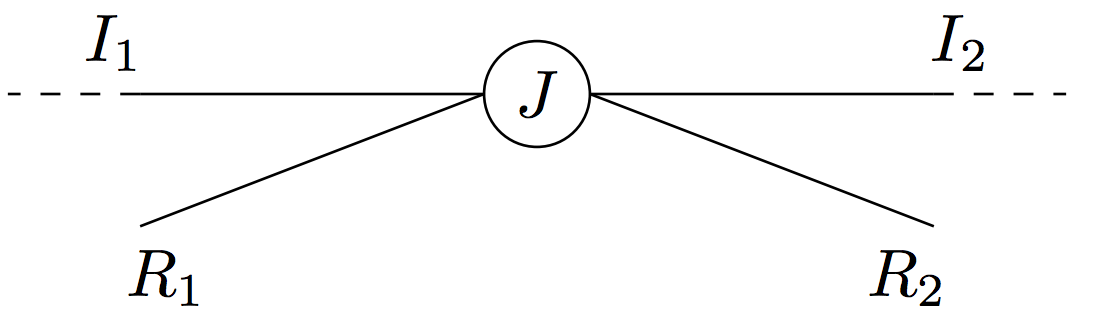
\includegraphics[width=0.6\textwidth]{diagrams/simple-junction}
	\caption{A freeway junction consisting of an upstream mainline $I_1$, downstream mainline $I_2$, onramp $R_1$ and offramp $R_2$.}
	\label{fig:simple-junction}
\end{figure}

\subsubsection{Weak Boundary Conditions and Vehicle Conservation}

In reality, one cannot consider the evolution of a stretch of freeway in complete isolation with respect to its surrounding traffic network, as the dynamics are coupled at every junction point via Riemann solvers (Section~\ref{sec:riemann-solvers}). Thus, to account for the behavior at the extremities of the network, one must consider boundary conditions.

The standard approach to boundary conditions is to prescribe a time-varying density $\rho^0\left(t\right)$ at each extremity point of the network. Due to the concave shape of the fundamental diagram of traffic, density waves may propagate from within the system outwards to the network extremities, in both the upstream and downstream directions.

As an example, one could consider the behavior upstream of onramp $R_1$ as being the solution of a Riemann problem of the form in Equation~\eqref{eqn:riemann-problem}, where $\rho_-$ is the upstream boundary condition, and $\rho_+$ is the state within an onramp. Whenever $f\left(\rho_+\right)<f\left(\rho_-\right)$ and $\rho_+ > \rho^{\text{cr}}$, then it can be shown~\cite{lebacque1996godunov,garavello2006traffic} that the vehicle flux across the boundary is $f\left(\rho_+\right)$ and is thus insensitive to the value of $f\left(\rho_-\right)$. One can view this event as a \emph{loss of information} at the left boundary of the network, as the backward-moving congestion wave prevented information about the boundary condition from entering the network. Systems which possess this property are said to have \emph{weak boundary conditions}~\cite{strub2006weak}.

This property of traffic network modeling is undesirable in traffic management applications, as the flux of vehicles at network boundaries is dependent upon the state of the system, which in turn is dependent upon the control scheme being applied. Summarizing, different control schemes can lead to different vehicle demands, which is not a realistic assumption, can actually be exploited by control schemes. As the goal of the current traffic model is to be used in control applications, we develop an alternative approach which effectively turns the weak boundary conditions into \emph{strong} boundary conditions which guarantee vehicle flux conservation.

\subsubsection{Onramps as ODE Buffers}

Instead of modeling boundary conditions as vehicle densities, we consider a time-varying boundary \emph{flux}, $\demandsym\left(t\right)$ entering onramp $R_1$ and make the simplifying assumption that the offramp $R_2$ has infinite capacity and thus does not influence the evolution of the system\footnote{Motivation behind the offramp model is the focus on ramp-metering applications in this thesis, and the general lack of available sensor data on freeway offramps, making accurate modeling of offramp state difficult.}.

The onramp $R_1$ stores the boundary flux in a vehicle \emph{buffer} modeled by the following ordinary differential equation (ODE):

\begin{equation}
\label{eqn:ode-buffer}
\Dfrac{l\left(t\right)}{t} = \demandsym\left(t\right) - r\left(t\right),\quad t\in \R^+,
\end{equation}

where $r$ is the flux of vehicles exiting the onramp onto the downstream mainline $I_2$.

The onramp ODE models the conservation of boundary flux in a \emph{vertical} buffer of infinite capacity, as opposed to a spatially distributed \emph{horizontal} queue with finite capacity, until there is enough capacity on the downstream mainline to empty the queue.

As the offramp $R_2$ possesses no state, it does not require an ODE buffer. The behavior of vehicles at the offramp is captured via a \emph{split ratio} parameter $\splitratio \left(t\right) \in \left[0,1\right]$ which specifies the fraction of vehicles which move from $I_1$ to $I_2$, where $1 - \splitratio\left(t\right)$ is the fraction of vehicles leaving the freeway from $I_1$ to $R_2$. It is assumed that no vehicles from $R_1$ immediately exit to $R_2$.

Thus, the Cauchy problem we wish to solve across the four-link system is as follows:

\begin{align}
\partial_t \rho_i + \partial_x f\left(\rho_i\right) = 0, & \quad \left(t,x\right) \in \R^+ \times I_i, \, i = 1,2 \\
\Dfrac{l\left(t\right)}{t} = \demandsym\left(t\right) - r\left(t\right), & \quad t\in \R^+ \\
\rho_i \left(0,x\right) = \rho_{i,0} \left(x\right), & \quad \text{On } I_i\, i = 1,2 \\
l\left(0\right) = l_0, &
\end{align}

where $\rho_{i,0}$ is the initial condition on the mainline links $I_i$ and $l_0$ is the initial number of vehicles in $R_1$.

\subsubsection{Riemann Solver for PDE-ODE Model}

We assume for our applications that the fundamental diagram has a trapezoidal form as depicted
in Fig.~\ref{fig:Fundamental-diagram-with}, where $v$ is the \emph{free-flow} speed of traffic and $w$ is referred to as the \emph{congestion wave} speed.

\begin{figure}
\centering
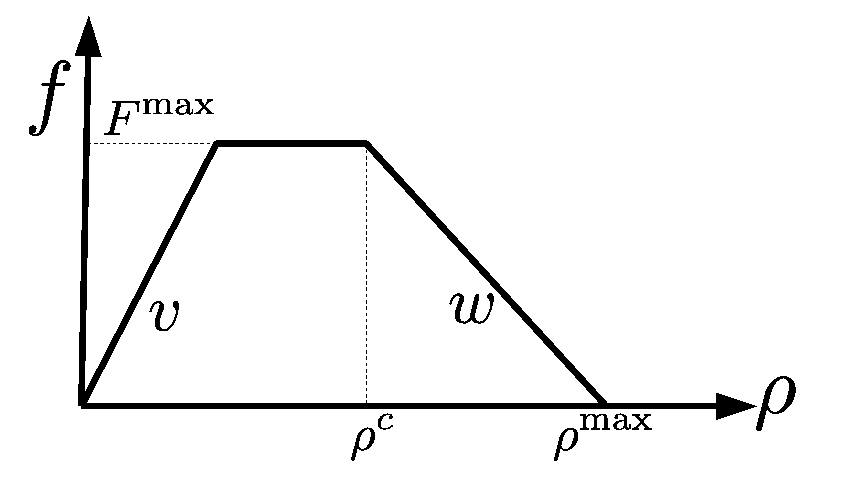
\includegraphics[width=0.4\columnwidth]{previous-articles/adjoint/figs-gen/fd}
\caption[Fundamental diagram with free-flow speed $v$, congestion wave speed $w$,
max flux $F^{\max}$, critical density $\density^{c}$, and max density
$\density^{\max}$.]{Fundamental diagram (the name of the flux function in transportation
literature) with free-flow speed $v$, congestion wave speed $w$,
max flux $F^{\max}$, critical density $\density^{c}$, and max density
$\density^{\max}$.\label{fig:Fundamental-diagram-with}}
\end{figure}

There are many potential Riemann solvers that satisfy the properties required in Section~\ref{sec:riemann-solvers}.
To guarantee a unique solution for each Riemann datum, we add two modeling decisions to solve the junction. Let $\rho_1^+$ and $\rho_2^-$ be the densities on $I_1$ and $I_2$ (respective) adjacent to the junction. Let $l$ be the queue length on $R_1$. Then let $\hat{\rho}_1^+$, $\hat{\rho}_2^-$ be the resulting Riemann solutions for $I_1$  and $I_2$, while $\hat{r}$ is the resulting Riemann flux from $R_1$. The additional modeling decisions are then:
\begin{enumerate}
\item The flux solution maximizes the outgoing mainline flux $f\left(\hat{\rho}_1^+\right)$
\item When (1) does not give a unique solution, the Riemann solver attempts to satisfy $f\left(\hat{\rho}_2^-\right)=p f\left(\hat{\rho}_1^+\right)$,
where $p\in\mathbb{R}_{+}$ is a merging parameter. The $p$ parameter sets the priority of flow from $I_1$ over the flow from $R_1$ when there is limited capacity. Since (1) permits multiple flux solutions at the junction, (2) is necessary to obtain a unique solution.
\end{enumerate}

With the necessary restrictions on the Riemann solver in place, we outline the solution method for the PDE-ODE junction problem. The well-posedness and self-similarity proofs are given in~\cite{delle2014pde}. The method closely follows that of general LWR network solutions presented in~\cite{garavello2006traffic}.

For a Riemann datum of $\left(\rho_1^+, \rho_2^-, l\right)$, we introduce the following intermediate variables:

\begin{itemize}
	\item $\delta = \min\left(F^{\max}, v \rho_1^+\right)$, the maximum allowable flux out of $I_1$.
	\item $d =
	\begin{cases}
	F^{\max} & \text{if } l > 0 \\
	\min\left(F^{\max}, D\left(t\right)\right) & \text{if } l = 0
	\end{cases}$, the maximum allowable flux out of $R_1$
	\item $\sigma = \min\left(F^{\max}, w \left(\rho^{\max} - \rho_2^-\right)\right)$, the maximum allowable flux into $I_2$.
\end{itemize}

The maximal flux into $I_2$ is computed as $f_2 = \min\left(\beta\delta + d, \sigma\right)$, the minimum between the upstream \emph{demand}, and the downstream \emph{supply}.

\begin{figure}[t]
\subfloat[Case 1: Priority violated due to limited upstream mainline demand
entering downstream mainline.]{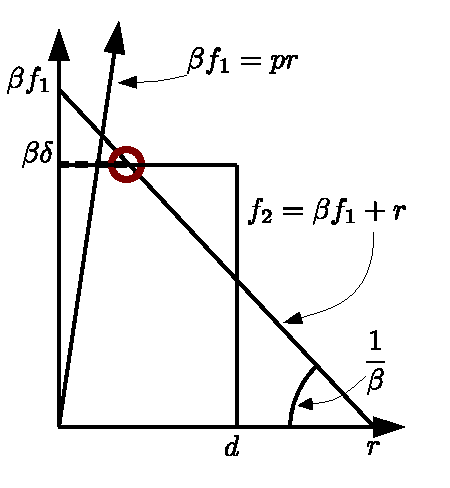
\includegraphics[width=0.25\columnwidth]{previous-articles/adjoint/figures/flux-sln-1}
}\hfill%
\subfloat[Case 2: Priority violated due to limited on ramp demand entering downstream
mainline.]{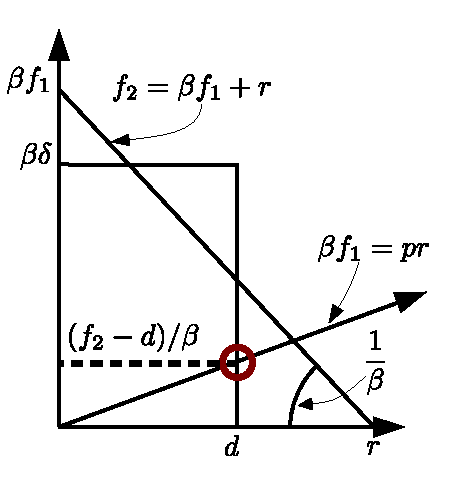
\includegraphics[width=0.25\columnwidth]{previous-articles/adjoint/figures/flux-sln-2-thesis}
}\hfill%
\subfloat[Case 3: Priority rule satisfied due to sufficient demand from both
mainline and on ramp.]{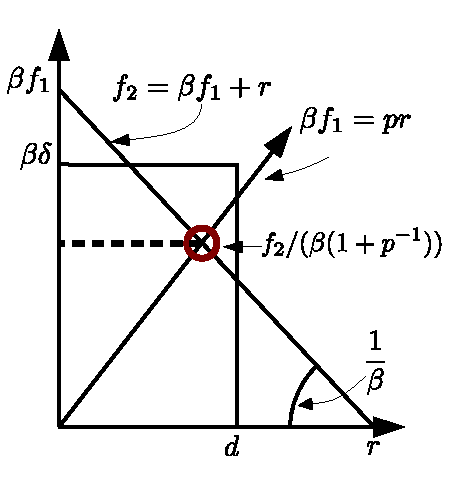
\includegraphics[width=0.25\columnwidth]{previous-articles/adjoint/figures/flux-sln-3-thesis}
}
\caption[Godunov junction flux solution for freeway model.]{Godunov junction flux solution for freeway model. The rectangular region represents the feasible flux
values for $I_1$ ($\beta \delta$) and $R_1$ ($d$) as determined by the upstream demand, while
the line with slope $\frac{1}{\beta}$
represents feasible flux values as determined by mass balance. The
$\beta f_1$
term accounts for only the flux out of $I_1$
that stays on the mainline. The flux solution, represented by the
red circle, is the point on the feasible region that minimizes the
distance from the priority line $f_1 = p r$.}
\label{fig:Godunov-junction-flux}
\end{figure}

To compute the flux leaving $I_1$, we refer to Figure~\ref{fig:Godunov-junction-flux}. The balance between the fluxes $\beta f_1$ (resp. $r$) entering $I_2$  from $I_1$ (resp. $R_1$) must minimize the deviation from the equation $\beta f_1 = p r$. Since flow must be conserved across the junction, we also have the constraint that the $\left(\beta f_1, r\right)$ flows must sum to $f_2$, and thus the resultant flow pair $\left(f_1, r\right)$ must lie on the line $f_2 = \beta f_1 + r$, depicted in Figure~\ref{fig:Godunov-junction-flux}. This results in three distinct cases for the $f_1$ solution.

\begin{itemize}
	\item In Case 1, strict satisfaction of the priority line would lead to an $f_1$ value greater than $\delta$ when at the intersection with the supply line $f_2 = \beta f_1 + r$. Since $\delta$ is the maximum allowable flux from $I_1$, we can feasibly exactly satisfy the priority. Thus to minimize the deviation from the priority line, we select $f_1 = \delta$.
	\item In Case 2, the priority dictates a flux from $R_1$ in excess of $d$. To minimize deviation from priority, we select $r = d$, and $\beta f_1 = f_2 - r$.
	\item In Case 3, strict satisfaction of the priority line gives a feasible $f_1$ and $r$ solution, and thus we have $f_1 = \frac{f_2}{\beta \left(1 + p^{-1}\right)}$.
\end{itemize}


Once we have determined $f_1$ and $f_2$, then flux balance across the junction dictates that $r = f_2 - \beta f_1$.

To satisfy the Riemann solver condition that only waves that travel outward from the junction may be created, we devise a mapping from the resultant mainline fluxes $\left(f_1, f_2\right)$ to the Riemann solver densities $\left(\hat{\rho}_1^+, \hat{\rho}_2^-\right)$. The following conditions uniquely determine $\left(\hat{\rho}_1^+, \hat{\rho}_2^-\right)$:

\begin{align}
\hat{\rho}_1^+ \in
\begin{cases}
\left\{\rho_1^+\right\}\cup ]\tau(\rho_1^+),\rho^{\max}] & \text{if } 0 \le \rho_1^+ \le \rho^\text{cr}, \\
\left[\rho^{\text{cr}}, \rho^{\max}\right] & \text{if }  \rho^\text{cr} \le  \rho_1^+ \le \rho^{\max};
\end{cases} &\quad  & f\left(\hat{\rho}_1^+\right) = f_1 \\
\hat{\rho}_2^- \in
\begin{cases}
\left[0,\rho^{\text{cr}}\right] & \text{if } 0 \le \rho_2^- \le \rho^\text{cr}, \\
 \left\{\rho_2^-\right\}\cup [0,\tau(\rho_2^-)]
 & \text{if }  \rho^\text{cr} \le  \rho_2^- \le \rho^{\max};
\end{cases} &\quad  & f\left(\hat{\rho}_2^-\right) = f_2,
\end{align}

where $\tau$ satisfies the following:

\begin{enumerate}
	\item $f(\tau(\rho)) = f(\rho)$
	\item $\tau(\rho) \neq \rho$
\end{enumerate}

\subsection{Discrete Freeway Model}

The previous section derives a continuous traffic model based on the principle of mass conservation and matching the empirical flux-density relationship. Furthermore, the model possesses strong boundary conditions, allowing for the total flux through the network to be independent of any varying control parameters.

In order to develop computationally efficient optimization and control techniques, we work in the discrete time and space domain. As detailed in Section~\ref{sec:godunov-discretization}, we use the Godunov discretization technique.

We now consider a freeway network with multiple junctions, as opposed to the presentation of the continuous model, which only considered a single junction.

Consider a freeway section with links $\links=\intrange 1{2\nlinks}$
with a linear sequence of mainline links $=\intrange{2,4}{2\nlinks}$
and connecting on ramp links $=\intrange{1,3}{2\nlinks-1}$. At discrete
time $t=\tind\Delta t,0\le\tind\le\ntime-1$, mainline link $2\link\in\links,i\in\intrange 1{\nlinks}$
has a downstream junction $\jdown{2\link}=\jup{2\left(\link+1\right)}$
and an upstream junction $\jup{2\link}=\jdown{2\left(\link-1\right)}$,
while on ramp $2\link-1\in\links,i\in\intrange 1{\nlinks}$ has a downstream
junction $\jdown{2\link-1}=\jup{2\link}=\jdown{2\left(\link-1\right)}$
and an upstream junction $\jup{2\link-1}$.

The off-ramp directly downstream of link $2\link,i\in\intrange 1{\nlinks}$
has, at time-step $\tind$, a split ratio $\splitratio_{2\link}^{\tind}$
Each link $\link\in\links$ has a discretized state value $\densitydiscrete{\link}{\tind}\in\mathbb{R}$
at each time-step $\tind\in\intrange 0{\ntime-1}$, that represents
the density of vehicles on the link. These values are depicted in
Fig~\ref{fig:Freeway-network-junction}. Junctions that have no
on ramps can be effectively represented by adding an on ramp with no
demand while junctions with no off-ramps can be represented by setting
the split ratio to 1.
\begin{figure}
\centering
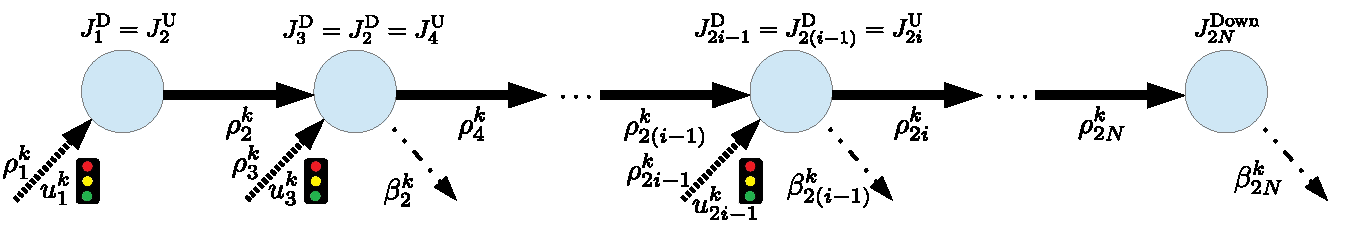
\includegraphics[width=1\columnwidth]{previous-articles/adjoint/figs-gen/rm-junction-2}
\caption[Freeway network model depicting the discrete model notation on a single freeway/onramp junction.]{Freeway network model. For a junction $\jdown{2\link-1}=\jdown{2\left(\link-1\right)}=\jup{2\link}$
at time-step $\tind\in\intrange 0{\ntime-1}$, the upstream mainline
density are represented by $\densitydiscrete{2\left(\link-1\right)}{\tind}$,
the downstream mainline density by $\densitydiscrete{2\link}{\tind}$,
the on ramp density by $\densitydiscrete{2\link-1}{\tind}$, and the
off-ramp split ratio by $\splitratio_{2\left(\link-1\right)}^{\tind}$.}
\label{fig:Freeway-network-junction}
\end{figure}

As control input which is used extensively in applications in proceeding sections, an on ramp $2\link-1\in\links,\link\in\intrange 1{\nlinks}$
at time-step $k\in\intrange 0{\ntime-1}$ has a metering rate $\ramp_{2\link-1}^{\tind}\in\left[0,1\right]$
which limits the flux of vehicles leaving the on ramp. Intuitively,
the metering rate acts as a fractional decrease in the flow leaving
the on ramp and entering the mainline freeway. The domain of the metering
control is to force the control to neither impose negative flows nor
send more vehicles than present in a queue. Its mathematical model
is expressed in~\eqref{eq:ramp-eqn}.

For notational simplicity we define the set of densities of links
incident to $\jup{2\link}=\jdown{2\left(\link-1\right)}$ at time-step
$\tind$ as $\juncstate{\jup{2\link}}{\tind}=\left\{ \discrete{2\left(\link-1\right)}{\tind},\discrete{2i-1}{\tind},\discrete{2\link}{\tind}\right\} $. For $k\in\intrange 1{\ntime-1}$,
the mainline density $\discrete{2\link}{\tind}$ using the Godunov
scheme from~\eqref{eq:godscheme} is given by:

\begin{eqnarray}
\syseq_{2\link}^{\tind}(\state,\control)= & \discrete{2\link}{\tind}-\discrete{2\link}{\tind-1} & +\dfrac{\Delta t}{\length_{2\link}}\left(\god_{\jdown{2\link}}\left(\juncstate{\jdown{2\link}}{\tind-1},\ramp_{2\link+1}^{\tind-1}\right)\right)_{2\link}\label{eq:rho-update}\\
&  & -\dfrac{\Delta t}{\length_{2\link}}\left(\god_{\jup{2\link}}\left(\juncstate{\jup{2\link}}{\tind-1},\ramp_{2\link-1}^{\tind-1}\right)\right)_{2\link}\nonumber \\
= & \discrete{2\link}{\tind}-\discrete{2\link}{\tind-1} & +\frac{\Delta t}{\length_{2\link}}\left(\fout{2\link}{\tind-1}-\fin{2\link}{\tind-1}\right)=0
\end{eqnarray}
where we have introduced some substitutions to reduce the notational
burden of this section: $\fout{\link}{\tind}$ is the Godunov flux
at time-step $\tind$ exiting a link $\link$ at the downstream boundary
of the link, and $\fin{\link}{\tind}$ is the Godunov flux entering
the link at the upstream boundary.

We also make the assumption that on ramps have infinite capacity and
a free-flow velocity $\ffspeed_{2\link-1}=\frac{\length_{2\link-1}}{\Delta t}$
to prevent the ramp congestion from blocking demand from ever entering
the network. Since the on ramp has no physical length, the length
is chosen arbitrarily and the ``virtual'' velocity chosen above
is chosen to replicate the dynamics in~\cite{delle2014pde}. We can
then simplify the on ramp update equation to be:

\begin{eqnarray}
\syseq_{2\link-1}^{\tind}(\state,\control) & = & \discrete{2\link-1}{\tind}-\discrete{2\link-1}{\tind-1}-\frac{\Delta t}{\length_{2\link-1}}\left(\left(\god_{\jup{2\link}}\left(\juncstate{\jup{2\link}}{\tind-1},\ramp_{2\link-1}^{\tind-1}\right)\right)_{2\link-1}-\boundaryDemand{2\link-1}{\tind-1}\right)\label{eq:on ramp-update}\\
& = & \discrete{2\link-1}{\tind}-\discrete{2\link-1}{\tind-1}-\frac{\Delta t}{\length_{2\link-1}}\left(\fout{2\link-1}{\tind-1}-\boundaryDemand{2\link-1}{\tind-1}\right)=0
\end{eqnarray}
where $\boundaryDemand{2\link-1}{\tind-1}$ is the on ramp \emph{flux
}demand, and the same notational simplification has been used for
the downstream flux. This formulation results in ``strong'' boundary
conditions at the on ramps which guarantees all demand enters the network.

The on ramp model in~\eqref{eq:on ramp-update} differs from~\cite{delle2014pde}
in that we model the on ramp as a discretized PDE with an infinite
critical density, while~\cite{delle2014pde} models the on ramp
as an ODE ``buffer''. While both models implement strong boundary
conditions, the discretized PDE model makes the freeway network more
aligned with the PDE network framework presented in this section.

\paragraph{Discrete Model Equations}



The following systems of equations give the flux
solution of the Riemann solver at time-step $k\in\intrange 1{\ntime-1}$
and junction $\jup{2\link}$ for $\link\in\intrange 1{\nlinks}$:

\begin{eqnarray}
\demand_{2\left(\link-1\right)}^{\tind} & = & \min\left(\ffspeed_{2\left(i-1\right)}\densitydiscrete{2\left(\link-1\right)}{\tind},F_{2\left(\link-1\right)}^{\max}\right)\label{eq:first-ramp}\\
\supply_{2\link}^{\tind} & = & \min\left(\congspeed_{2i}\left(\density_{2i}^{\max}-\densitydiscrete{2\link}{\tind}\right),F_{2i}^{\max}\right)\label{eq:supply}\\
\rampDemand_{2\link-1}^{\tind} & = & \ramp_{2\link-1}^{\tind}\min\left(\frac{\length_{2\link-1}}{\Delta t}\densitydiscrete{2\link-1}{\tind},F_{2i-1}^{\max}\right)\label{eq:ramp-eqn}\\
\fin{2\link}{\tind} & = & \min\left(\splitratio_{2\left(\link-1\right)}^{\tind}\demand_{2\left(\link-1\right)}^{\tind}+\rampDemand_{2\link-1}^{\tind},\supply_{2\link}^{\tind}\right)\label{eq:fin}\\
\fout{2\left(\link-1\right)}{\tind} & = & \begin{cases}
\demand_{2\left(\link-1\right)}^{\tind} & \frac{p_{2(\link-1)}\fin{2\link}{\tind}}{\splitratio_{2\left(\link-1\right)}^{\tind}\left(1+p_{2(\link-1)}\right)}\ge\demand_{2\left(\link-1\right)}^{\tind}\hfill\text{[Case 1]}\\
\frac{\fin{2\link}{\tind}-\rampDemand_{2\link-1}^{\tind}}{\splitratio_{2\left(\link-1\right)}^{\tind}} & \frac{\fin{2\link}{\tind}}{1+p_{2(\link-1)}}\ge\rampDemand_{2\link-1}^{\tind}\hfill\text{[Case 2}]\\
\frac{p_{2(\link-1)}\fin{2\link}{\tind}}{\left(1+p_{2(\link-1)}\right)\splitratio_{2\left(\link-1\right)}^{\tind}} & \text{otherwise}\hfill[\text{Case 3]}
\end{cases}\label{eq:merge}\\
\fout{2\link-1}{\tind} & = & \fin{2\link}{\tind}-\splitratio_{2\left(\link-1\right)}^{\tind}\fout{2\left(\link-1\right)}{\tind}\label{eq:last-ramp}
\end{eqnarray}
where, for notational simplicity, at the edges of of the range for
$\link$, any undefined state values (e.g. $\densitydiscrete 0{\tind}$)
are assumed to be zero by convention. 

Note that the equations can be solved sequentially via forward substitution. Also, we do not include
the flux result for off-ramps explicitly here since its value has no
bearing on further calculations, and we will henceforth ignore its
calculation. To demonstrate that indeed the flux solution satisfies
the flux conservation property, the off-ramp flux is trivially determined
to be $\splitratio_{2\left(\link-1\right)}^{\tind}\fout{2\left(\link-1\right)}{\tind}$.
